\documentclass[11pt]{article}
\usepackage[a4paper,margin=1in]{geometry}
\usepackage{amsmath,amssymb,amsthm,mathtools}
\usepackage{hyperref}
\usepackage{physics}
\usepackage{enumitem}
\usepackage{tikz}
\usetikzlibrary{arrows.meta,calc,decorations.pathreplacing}

\title{Weierstrass Elliptic Function from \(dz\) and \(\dfrac{dz}{z}\)}
\author{}
\date{}

\newtheorem{definition}{Definition}
\newtheorem{fact}{Fact}
\newtheorem{theorem}{Theorem}
\newtheorem{exercise}{Exercise}

\begin{document}
	\maketitle
	
	\tableofcontents
	
	\section{From \(dz\) on \(\mathbb C\) to a torus \(X=\mathbb C/\Lambda\)}
	Fix two non-collinear complex numbers \(\omega_1,\omega_2\) and the lattice
	\[
	\Lambda=\mathbb Z\omega_1+\mathbb Z\omega_2.
	\]
	Identify \(z\sim z+\lambda\) for \(\lambda\in\Lambda\). The quotient \(X=\mathbb C/\Lambda\) is a complex torus.  
	The 1-form \(\omega=dz\) is holomorphic on \(\mathbb C\) and \(\Lambda\)-invariant, hence descends to a holomorphic 1-form on \(X\). By Liouville, it is unique up to a constant; crucially, it has \emph{no zeros}.
	
	\begin{center}
		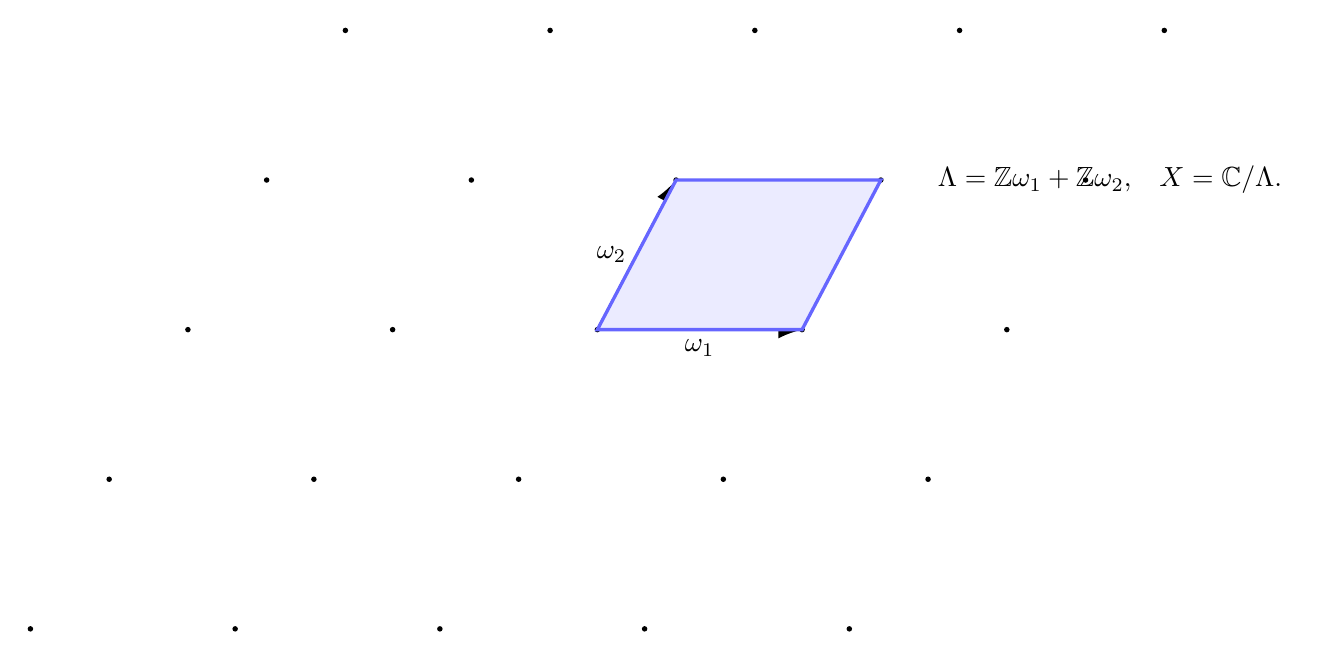
\begin{tikzpicture}[scale=1.0]
			% lattice
			\def\wone{2.6} \def\wtwoX{1.0} \def\wtwoY{1.9}
			\foreach \m in {-2,-1,0,1,2}{
				\foreach \n in {-2,-1,0,1,2}{
					\fill ({\m*\wone + \n*\wtwoX},{\n*\wtwoY}) circle (0.035);
				}
			}
			\draw[thick,-{Latex[length=3mm]}] (0,0) -- (\wone,0) node[midway,below] {$\omega_1$};
			\draw[thick,-{Latex[length=3mm]}] (0,0) -- (\wtwoX,\wtwoY) node[midway,left] {$\omega_2$};
			\coordinate (A) at (0,0);
			\coordinate (B) at (\wone,0);
			\coordinate (C) at ({\wone+\wtwoX},{\wtwoY});
			\coordinate (D) at (\wtwoX,\wtwoY);
			\fill[blue!8] (A)--(B)--(C)--(D)--cycle;
			\draw[blue!60,very thick] (A)--(B)--(C)--(D)--cycle;
			\node[align=left,anchor=west] at ($(C)+(0.6,0)$)
			{\(\Lambda=\mathbb Z\omega_1+\mathbb Z\omega_2\),\quad \(X=\mathbb C/\Lambda\).};
		\end{tikzpicture}
	\end{center}
	
	\section{Elliptic = periodic meromorphic; why no simple poles}
	\begin{definition}
		A function \(f:\mathbb C\to\mathbb C\) is \emph{elliptic} (w.r.t.\ \(\Lambda\)) if it is meromorphic and \(\Lambda\)-periodic:
		\(f(z+\lambda)=f(z)\) for all \(\lambda\in\Lambda\).
	\end{definition}
	
	There are no nonconstant \emph{holomorphic} elliptic functions (Liouville on a fundamental parallelogram), so any nontrivial elliptic \(f\) must have poles. Use the winding form \(\dfrac{dz}{z}\) to control residues:
	
	\begin{fact}[Residues in a fundamental domain]
		Let \(P\) be a fundamental parallelogram for \(\Lambda\). For an elliptic \(f\),
		\[
		\iint_{\partial P} f(z)\,dz \;=\; 2\pi i\!\!\sum_{\text{poles }a\in P}\!\!\mathrm{Res}_a(f)
		\quad\text{but}\quad
		\iint_{\partial P} f(z)\,dz=0
		\]
		because opposite edges cancel by periodicity. Hence \(\sum \mathrm{Res}_a(f)=0\).
	\end{fact}
	
	If an elliptic \(f\) had a \emph{single} simple pole in \(P\), its residue would have to be zero, forcing the principal part to vanish—contradiction. Therefore the “smallest” possible principal part is a \emph{double} pole with zero residue. That points us to a canonical choice.
	
	\section{Definition of the Weierstrass \texorpdfstring{\(\wp\)}{wp}}
	We choose the unique even elliptic function with a double pole at the lattice points and no constant term in its Laurent expansion at \(0\):
	\[
	\boxed{\;
		\wp(z;\Lambda)
		=\frac{1}{z^2}
		+\sum_{\substack{\omega\in\Lambda\\ \omega\neq 0}}
		\left(\frac{1}{(z-\omega)^2}-\frac{1}{\omega^2}\right)
		\;}
	\]
	The subtraction \(1/\omega^2\) kills the constant term and ensures normal convergence.
	
	\paragraph{Immediate properties.}
	\begin{itemize}[leftmargin=1.6em]
		\item \textbf{Double periodic:} \(\wp(z+\omega_j)=\wp(z)\) for \(j=1,2\).
		\item \textbf{Even:} \(\wp(-z)=\wp(z)\) (the summand is even).
		\item \textbf{Poles:} Only at \(\Lambda\), all \emph{double} with principal part \(1/z^2\).
		\item \(\wp'\) is \emph{odd} and elliptic, with \emph{triple} poles at \(\Lambda\).
	\end{itemize}
	
	\begin{center}
		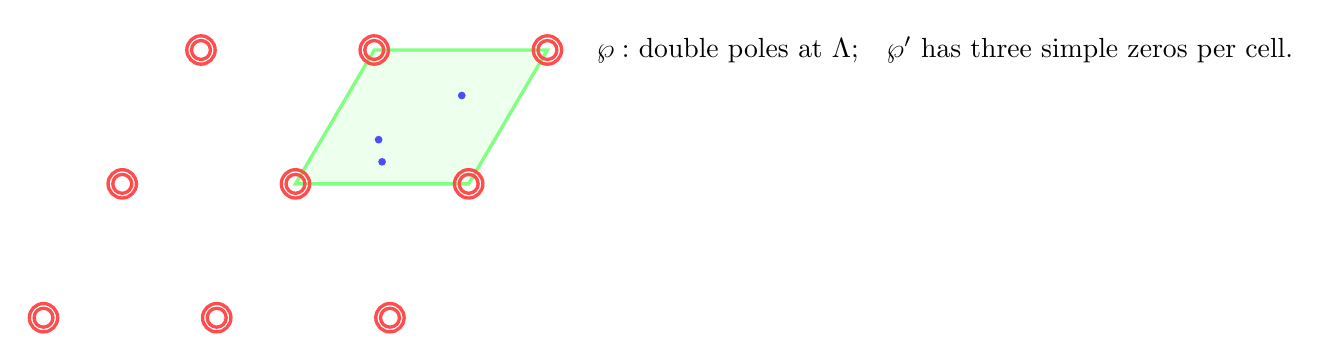
\begin{tikzpicture}[scale=1.0]
			% lattice and marking poles/zeros schematically
			\def\wone{2.2} \def\wtwoX{1.0} \def\wtwoY{1.7}
			% fundamental cell
			\coordinate (A) at (0,0);
			\coordinate (B) at (\wone,0);
			\coordinate (C) at ({\wone+\wtwoX},{\wtwoY});
			\coordinate (D) at (\wtwoX,\wtwoY);
			\fill[green!7] (A)--(B)--(C)--(D)--cycle;
			\draw[green!50,very thick] (A)--(B)--(C)--(D)--cycle;
			% lattice points as double poles
			\foreach \m in {-1,0,1}{
				\foreach \n in {-1,0,1}{
					\coordinate (P) at ({\m*\wone + \n*\wtwoX},{\n*\wtwoY});
					\draw[red!70,very thick] (P) circle (0.12);
					\draw[red!70,very thick] (P) circle (0.18);
				}
			}
			% schematic zeros of \wp' inside a cell (three simple zeros)
			\fill[blue!70] ($(A)!0.33!(C)$) circle (1.4pt);
			\fill[blue!70] ($(A)!0.66!(C)$) circle (1.4pt);
			\fill[blue!70] ($(A)!0.5!(B)$)++(0,0.28) circle (1.4pt);
			\node[align=left,anchor=west] at ($(C)+(0.5,0)$)
			{\(\wp:\) double poles at \(\Lambda\);\quad \(\wp'\) has three simple zeros per cell.};
		\end{tikzpicture}
	\end{center}
	
	\section{Laurent series and Eisenstein series}
	Expanding at \(z=0\) gives
	\[
	\wp(z)
	=\frac{1}{z^2}+\frac{g_2}{20}\,z^2+\frac{g_3}{28}\,z^4+\cdots,
	\qquad
	\wp'(z)=-\frac{2}{z^3}+\frac{g_2}{10}\,z+\frac{g_3}{7}\,z^3+\cdots
	\]
	where the lattice invariants are
	\[
	g_2=60\!\!\sum_{\omega\in\Lambda\setminus\{0\}}\frac{1}{\omega^4},
	\qquad
	g_3=140\!\!\sum_{\omega\in\Lambda\setminus\{0\}}\frac{1}{\omega^6}.
	\]
	(These are built from the holomorphic data of the lattice; note how only \(dz\) and the lattice enter.)
	
	\section{The cubic and the differential equation}
	Consider the cubic curve
	\[
	E:\quad y^2=4x^3-g_2x-g_3,\qquad \omega_E=\frac{dx}{y}.
	\]
	Define the \emph{Abel map} \(z=\displaystyle \int_{\infty}^{(x,y)}\omega_E\). Then the inverse map is
	\[
	\boxed{\;x=\wp(z),\qquad y=\wp'(z)\;}
	\]
	and the pair \((\wp(z),\wp'(z))\) automatically satisfies the cubic equation. Equivalently, one shows
	\[
	\boxed{\;\big(\wp'(z)\big)^2 = 4\big(\wp(z)\big)^3 - g_2\,\wp(z) - g_3\;}
	\]
	by observing that the left-hand side is an elliptic function with no poles (hence constant), and matching its Laurent expansion at \(0\) to force the constant to be \(0\).
	
	\begin{center}
		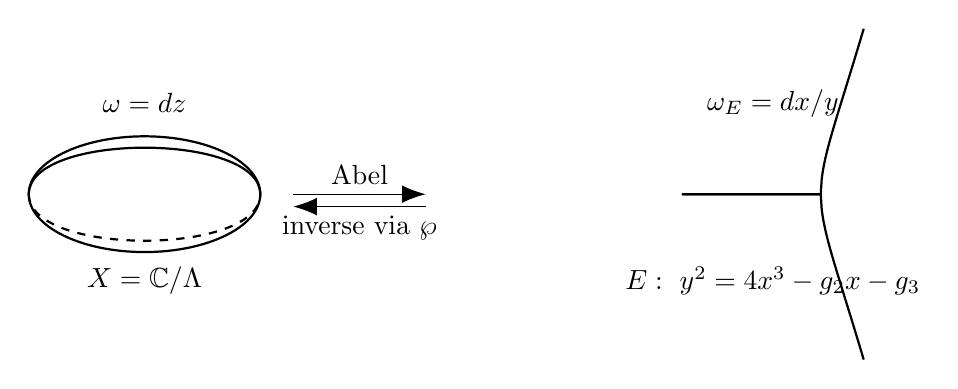
\begin{tikzpicture}[scale=1.05]
			% schematic dictionary: torus <-> cubic
			% Torus panel
			\begin{scope}[shift={(-4.0,0)}]
				\draw[thick] (0,0) ellipse (1.4 and 0.7);
				\draw[thick] (-1.4,0) .. controls (-1.4,0.75) and (1.4,0.75) .. (1.4,0);
				\draw[thick,dashed] (-1.4,0) .. controls (-1.4,-0.75) and (1.4,-0.75) .. (1.4,0);
				\node at (0,-1.05) {$X=\mathbb C/\Lambda$};
				\node at (0,1.1) {$\omega=dz$};
			\end{scope}
			% Arrow
			\draw[-{Latex[length=3mm]}] (-2.2,0) -- (-0.6,0) node[midway,above]{Abel};
			\draw[-{Latex[length=3mm]}] (-0.6,-0.15) -- (-2.2,-0.15) node[midway,below]{inverse via \(\wp\)};
			% Cubic panel
			\begin{scope}[shift={(3.6,0)}]
				% rough cubic shape
				\draw[thick,domain=-1.1:1.1,samples=200] plot(\x,{sqrt(max(0,4*\x*\x*\x - 1.0*\x - 0.2))});
				\draw[thick,domain=-1.1:1.1,samples=200] plot(\x,{-sqrt(max(0,4*\x*\x*\x - 1.0*\x - 0.2))});
				\node at (0,-1.05) {$E:\ y^2=4x^3-g_2x-g_3$};
				\node at (0,1.1) {$\omega_E=dx/y$};
			\end{scope}
		\end{tikzpicture}
	\end{center}
	
	\section{Periods, zeros, and the zeta primitive}
	Let \(2\omega_1,2\omega_2\) be a \emph{period basis} (\(\Lambda=2\omega_1\mathbb Z+2\omega_2\mathbb Z\)). Then \(\wp\) has those same periods; \(\wp'\) has three simple zeros in each fundamental domain (at half-periods when the lattice is generic). Define the Weierstrass zeta function by
	\[
	\zeta'(z)=-\wp(z),\qquad
	\zeta(z)=\frac{1}{z}+\!\!\sum_{\omega\neq 0}\!\left(\frac{1}{z-\omega}+\frac{1}{\omega}+\frac{z}{\omega^2}\right).
	\]
	It is \emph{not} elliptic (it has quasi-periods), reflecting the fact that a global primitive of \(\wp\) cannot be doubly periodic—compare with \(\log z\) for \(dz/z\).
	
	\section{Everything came from \(dz\) and \(\frac{dz}{z}\)}
	\begin{itemize}[leftmargin=1.6em]
		\item \(dz\) gives the unique holomorphic 1-form on the torus and defines periods.
		\item Elliptic \(=\) doubly periodic meromorphic; Stokes + periodicity + \(dz/z\) (residue calculus) force double poles and zero total residue.
		\item Killing the constant term canonically produces \(\wp\).
		\item The cubic relation arises because the pole-free combination must be constant.
	\end{itemize}
	
	\section*{Quick exercises}
	\begin{exercise}
		Show that if \(f\) is elliptic then \(\sum\mathrm{Res}(f)=0\) in a fundamental domain; deduce there is no elliptic function with exactly one simple pole.
	\end{exercise}
	\begin{exercise}
		Expand \(\wp(z)\) from the definition and read off the coefficients \(g_2/20\) and \(g_3/28\).
	\end{exercise}
	\begin{exercise}
		Prove \(\big(\wp'\big)^2-4\wp^3+g_2\wp+g_3\) is elliptic with no poles and use the Laurent expansions to conclude it vanishes identically.
	\end{exercise}
	
\end{document}
